\documentclass[pdf, aspectratio=169, 12pt]{beamer}
\usepackage[]{hyperref, graphicx, siunitx, lmodern, tikz, booktabs, physics}
\usepackage[mode=buildnew]{standalone}
\usepackage{pdfpc-commands}

\usetheme[sols]{Python}

\graphicspath{ {Images/} }

\sisetup{per-mode=symbol}
\usetikzlibrary{calc, patterns, decorations.markings, decorations.pathmorphing, shapes}

%Preamble
\title{If Strings Exist}
\author{Jed Rembold}
\date{January 29, 2020}

\begin{document}

\begin{frame}{Announcements}
	\begin{itemize}
		\item Homework 1 due Friday night
			\begin{itemize}
				\item Problems given in pdf
				\item Link to add template repository is also in pdf
					\begin{itemize}
						\item \alert{Download} the repository to your own system to work on locally!
					\end{itemize}
				\item Some extra guidelines in the repository README
				\item Demo of automatic testing here in a moment
			\end{itemize}
		\item Polling: \url{rembold-class.ddns.net}
	\end{itemize}
\end{frame}

\begin{frame}{Testing Demo}
	\begin{itemize}
		\item There is some automatic testing built in to the homework repositories
		\item Requires no extra effort on your part aside from not messing with special code I've written
		\item Gives you some idea if your code is generally behaving as intended
		\item Works on the \emph{entire} repository, so everything needs to be good to get a green passing badge on the README
		\item Can see a breakdown of which tests failed by following details (see demo)
		\item Can also view tests in VSCode
			\begin{itemize}
				\item Select PYTEST the first time when prompted, then menu on left
			\end{itemize}
	\end{itemize}
\end{frame}

\begin{frame}[fragile]{All things must change}
	\vspace{5mm}
	\begin{itemize}
		\item You can \alert{rebind} variables using a new assignment statement
		\item Old value gets lost
		\item Variables only change upon assignment. Changing something that a variable depends on does \emph{not} update that variable.
	\end{itemize}
	\begin{columns}
		\column{0.5\textwidth}
		\begin{pythoncode}[]
			|pi = 3.14159|
			|radius = 4|
			|circ = 2 * pi * radius|
			|radius = radius + 2|
		\end{pythoncode}
		
		\column{0.5\textwidth}
		\begin{center}
			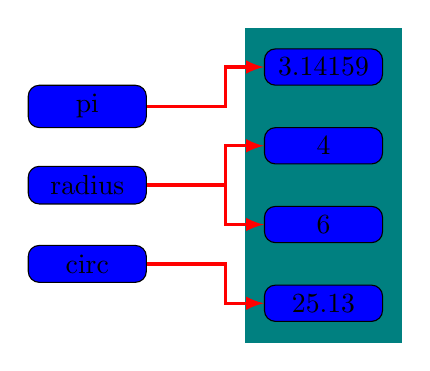
\begin{tikzpicture}[
				label/.style={rounded corners, draw=black, fill=Blue, text=black, minimum width=1.5cm}
				]
				\fill[Teal] (0,0) rectangle + (2,4);
				\node<1->[label](pinum) at (1,3.5) {3.14159};
				\node<2->[label](radnum) at (1,2.5) {4};
				\node<4->[label](radnum2) at (1,1.5) {6};
				\node<3->[label](circnum) at (1,0.5) {25.13};

				\node<1->[label](pi) at (-2,3) {pi};
				\node<2->[label](rad) at (-2,2) {radius};
				\node<3->[label](circ) at (-2,1) {circ};

				\draw<1->[Red, very thick, -latex] (pi.east) -- +(1,0) |- (pinum.west);
				\draw<2-3>[Red, very thick, -latex] (rad.east) -- +(1,0) |- (radnum.west);
				\draw<4->[Red, very thick, -latex] (rad.east) -- +(1,0) |- (radnum2.west);
				\draw<3->[Red, very thick, -latex] (circ.east) -- +(1,0) |- (circnum.west);

			\end{tikzpicture}
		\end{center}
	\end{columns}
\end{frame}

\begin{frame}[fragile]{Two other \#Comments}
	\vspace{5mm}
	\begin{itemize}
		\item You can assign multiple variables at the same time
			\begin{pythoncode}
				x, y = 5, 10	
			\end{pythoncode}
			\begin{itemize}
				\item This can be useful for swapping variables, since everything gets evaluated before the bindings are assigned
					\begin{pythoncode}
						x, y = y, x
					\end{pythoncode}
			\end{itemize}
		\item Use comments in your code to explain otherwise confusing or unclear sections
			\begin{pythoncode}
				#This is a comment
				#The interpreter will completely ignore these
				#lines while the code is being executed
				4 + 5
			\end{pythoncode}
	\end{itemize}
\end{frame}

\begin{frame}[fragile]{Understanding Check}
	What is the final printed value of \pyi{A} in the code below?
	\begin{pythoncode}[numbers=left]
		A = 10
		B = 4
		C = A * B
		A = C - A
		# B = A
		A, B, C = C, A, B
	\end{pythoncode}
	\begin{poll}
	\item 4
	\item 10
	\item 30
	\item 40
	\end{poll}
	\exsol{40}
\end{frame}

\begin{frame}{Moving beyond making calculators}
	\begin{columns}
		\column{0.5\textwidth}
		\begin{itemize}
			\item Recall that a requirement of an algorithm is that it has some sort of flow control
			\item Thus far, everything we've done or looked at proceeds in a straight line%
				\begin{itemize}
					\item Simple, but inherently boring
					\item Not much you can do with it beyond basic calculations
				\end{itemize}
			\item Want to talk now about how to write branching programs
		\end{itemize}
		
		\column{0.5\textwidth}
		\begin{center}
			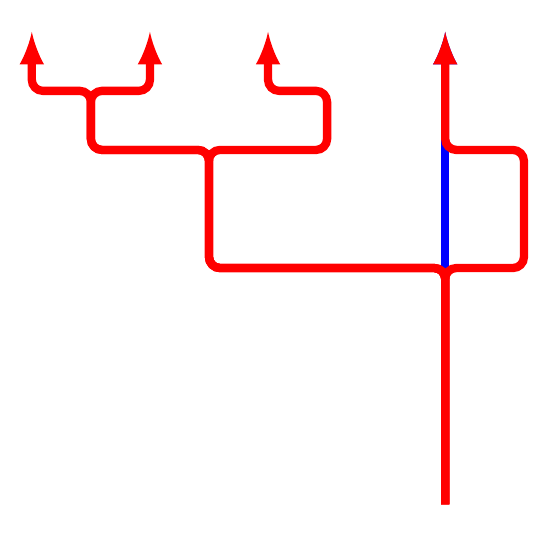
\begin{tikzpicture}
				\draw[line width=3pt, -latex, Blue] (0,0) -- +(0,6);
				\onslide<2>{
					\draw[line width=3pt, -latex, Red, rounded corners]
						(0,0) |- ++(-3,3) |- ++(-1.5,1.5) |- ++(-.75,.75) -- ++(0,.75);
					\draw[line width=3pt, -latex, Red, rounded corners]
						(0,0) |- ++(-3,3) |- ++(1.5,1.5) |- ++(-.75,.75) -- ++(0,.75);
					\draw[line width=3pt, -latex, Red, rounded corners]
						(0,0) |- ++(-3,3) |- ++(-1.5,1.5) |- ++(.75,.75) -- ++(0,.75);
					\draw[line width=3pt, -latex, Red, rounded corners]
						(0,0) |- ++(1,3) |- ++(-1,1.5) -- ++(0,1.5);
				}
			\end{tikzpicture}
		\end{center}
	\end{columns}
\end{frame}

\begin{frame}{The Conditional}
	\begin{center}
		\begin{tikzpicture}[
			block/.style={rounded corners, draw, very thick, fill=Orange, minimum width=2cm, minimum height=1cm, font=\Large, text=BG},
			choice/.style={rounded corners, draw, very thick, fill=Blue, minimum width=2cm, minimum height=1cm, font=\Large, diamond, text=BG}
			]
			\draw[line width=3pt, Purple] (2.5,-3) rectangle (9,3);

			\node[block](c1) at (0,0) {Code};
			\node[choice](t) at (4,0) {Test};
			\node[block, fill=Teal](true) at (6,2) {True Block};
			\node[block, fill=Red](false) at (6,-2) {False Block};
			\node[block](c2) at (11,0) {Code};

			\draw[ultra thick, -latex] (c1.east) -- (t.west);
			\draw[ultra thick, -latex, Teal] (t.north) |- (true.west);
			\draw[ultra thick, -latex, Red] (t.south) |- (false.west);
			\draw[ultra thick, -latex] (true.east) -| ($(c2.west)-(2,0)$) -- (c2.west);
			\draw[ultra thick, -latex] (false.east) -| ($(c2.west)-(2,0)$) -- (c2.west);
		\end{tikzpicture}
	\end{center}
\end{frame}

\begin{frame}[fragile]{Python Conditional Syntax}
	\vspace{5mm}
	In Python, the basic conditional looks like:
	\begin{pythoncode}
		if boolean_expression:
			# True block of code
			# Code to run if the test is true
		else:
			# False block of code
			# Code to run if the test is false
	\end{pythoncode}

	\begin{itemize}
		\item Things to note:
			\begin{itemize}
				\item A colon \pyi{:} ends each of the \pyi{if} and \pyi{else} lines
				\item True and False blocks are \alert{indented}
				\item You do not need an \pyi{else} portion if your desired false block is empty
				\item Boolean expression can be anything that evaluates to True/False
			\end{itemize}
	\end{itemize}
\end{frame}

\begin{frame}{Tests}
	\begin{itemize}
		\item Tests can be any expression that returns a Boolean, but common ones are:
			\begin{itemize}
				\item \pyi{==} \hspace{5mm} check if two things are equal
				\item \pyi{ >} \hspace{5mm} check if something is greater than the other
				\item \pyi{ <} \hspace{5mm} check if something is less than the other
				\item \pyi{>=} \hspace{5mm} check if something is greater than or equal to the other
				\item \pyi{<=} \hspace{5mm} check if something is less than or equal to the other
				\item \pyi{!=} \hspace{5mm} check if two things are not equal
			\end{itemize}
	\end{itemize}
\end{frame}

\begin{frame}[fragile]{Compounds and Nests}
	You can check multiple conditions in a variety of ways
	\begin{columns}[t]
		\column{0.5\textwidth}
		\begin{itemize}
			\item Nested Conditionals
		\end{itemize}
		\begin{pythoncode}[tabsize=2]
			if num%3 == 0:
				if num%4 == 0:
					print("Divisible by 3 and 4")
				else:
					print("Divisible by 3")
		\end{pythoncode}
		\column{0.5\textwidth}
		\begin{itemize}
			\item Compound Conditionals
		\end{itemize}
		\begin{pythoncode}
			if num%3==0 and num%4==0:
				print("Divisible by 3 and 4")
		\end{pythoncode}
	\end{columns}
\end{frame}

\begin{frame}[fragile]{Mr Elif}
	\vspace{5mm}
	\begin{itemize}
		\item A common issue that arises is when one condition is false (so you'd move to the false block) but then you immediately want to check another condition
		\item Python has a shorthand for this: the \pyi{elif}
	\end{itemize}
	\begin{pythoncode}
		if animal == "Dog":
			print("Woof!")
		elif animal == "Cat":
			print("Meow!")
		elif animal == "Bird":
			print("Tweet!")
		elif animal == "Fox":
			print("Ring-ding-ding-ding-dingeringeding!")
	\end{pythoncode}
	\begin{itemize}
		\item Usually want mutually exclusive things: something can't be both
	\end{itemize}
\end{frame}

\begin{frame}[fragile]{Understanding Check}
	\begin{columns}
		\column{0.6\textwidth}
		\vspace{3mm}
		\begin{pythoncode}[basicstyle=\footnotesize\ttfamily]
			animal = "shark"
			number = 5

			if animal == "kitten":
				if number > 10:
					print("I am in heaven!")
				else:
					print("I am still happy!")
			elif animal == "goat" and number > 5:
				print("This is getting excessive.")
			if animal == "shark":
				if number > 0:
					print("This is the worst day.")
			else:
				print("Today is an ok day.")
		\end{pythoncode}
		
		\column{0.4\textwidth}
		What will be printed to the screen if the code to the left is run?
		\begin{poll}
		\item This is getting excessive.
		\item Today is an ok day.
		\item I am still happy!
		\item Nothing printed to screen
		\end{poll}
	\end{columns}
	\exsol{Nothing printed to screen}
\end{frame}

\begin{frame}[fragile]{String Theory}
	\begin{itemize}
		\item Our first non-scalar object type
		\item Comprised of multiple characters
		\item Enclosed in either single or double quotes
			\begin{pythoncode}
				"This is a string!"
				'This is also a string.'
			\end{pythoncode}
	\end{itemize}
\end{frame}

\begin{frame}{Stringy Operations}
	\begin{itemize}
		\item \pyi{'a' + 'a'} \alert{concatenates} strings to give \pyi{'aa'}
		\item \pyi{3 * 'ha'} \alert{repeats} strings to give \pyi{'hahaha'}
		\item \pyi{len('fish')} will give the \alert{length} of the string (4 here)
		\item Comparisons check that all parts of the string match
			\begin{itemize}
				\item \pyi{'fish' == 'Fish'} will return \pyi{False}
			\end{itemize}
		\item Be careful of \pyi{<} or \pyi{>} comparisons of strings
			\begin{itemize}
				\item Generally work alphabetically
				\item But any capital letter at the \emph{start} is ``less'' than a lowercase letter
			\end{itemize}
	\end{itemize}
\end{frame}

\begin{frame}[fragile]{Getting Your Input}
	\begin{itemize}
		\item We already have \pyi{print()} for writing things to the terminal
		\item How can we give the program some sort of input short of editing the code?
			\begin{itemize}
				\item One method is the aptly named \pyi{input()} function
				\item Gives you a \alert{prompt} at the terminal to enter something
					\begin{pythoncode}
						guess = input('Guess any number between 1 and 10: ')
					\end{pythoncode}
				\item Always returns a \alert{string}, so further conversion may be necessary
			\end{itemize}
	\end{itemize}
\end{frame}





\end{document}

